\section{Virtual Sensor Field}
\label{chap:formulation}
The key element in designing a distributed Virtual Sensor Field is to find the optimal group of sensors that can approximate the missing ones through data driven machine learning.
The system evaluates the error generated by the approximation on multiple operational objectives to yield a minimalist set of possible solutions.
Each solution is then interpreted as a set of locations to place sensors along with their types. 

\subsection{Sensor Grouping}

Let assume there are a maximum of K types of sensors in the building, which are grouped according to their nature like groups of temperature, humidity, power sensors etc.
We will interpret the function $A^c(g)$ to fetch elements of a group $g$ from a chromosome. 
So for a sensor-wise grouping, we set the access function $A^c(g) =A_s^c(g)$ for $g \in K$ groups as 
\begin{equation}
    A_s^c(g \in K) = \{e_g^z | \forall z \in Z\}
\end{equation}
Spatial grouping of sensors is done by setting $A^c(g) =A_z^c(g)$ to partition the sensor set as shown in Equation \ref{eq:zonalChromosome}. 
\begin{equation}
    A_z^c(g \in Z) = \{e_i^g | \forall i \in K\}
    \label{eq:zonalChromosome}
\end{equation}


We construct \textbf{building chromosome} $B^c$ as an aggregation of (G) logical groups such that $|B^c| = \Sigma_{g \in G}|A^c(g)|$ as per Equation \ref{eq:chromosome}. 
The 1D vector of 0's and 1's represent offline/missing or online status of sensors respectively and is constructed by appending $A^c(g)$ in any arbitrary fixed order of $g \in Z \lor K$.
\begin{equation}
B^c = \{e^i_1, e^i_2 \dots e^i_K\} \forall i \in G, e^i_j \in \{0,1\}
\label{eq:chromosome}
\end{equation}


\subsection{Virtual Field }

Within a group, the subgroup denoted by \textbf{0} encoding is treated as the approximation set $A_g$ and the rest of sensors as support set $S_g$.
The collective task for a group $g$ is to learn the best mapping $\mathcal{H}^*$ from $S_g \xrightarrow[]{\mathcal{H}^*} A_g$.
%
The hypothesis space given by Equation  composed of two parts, to support bidirectional mapping between sets $\{A_g, S_g\}$
 \begin{equation}
  \mathcal{H}^g=\begin{bmatrix}
 \mathcal{H}^g_{f} &: S_g \rightarrow A_g  \\
 \mathcal{H}^g_{b} &: A_g \rightarrow S_g
 \end{bmatrix}
 \label{eq:recalibSet}
 \end{equation}
For the $g^{th}$ group, we store a 2D \textbf{error matrix} ${M}^g$ and a \textbf{library} $\mathcal{H}^g$ of machine learnt functions, both of size $|A^c(g)|^2$.
A function $L$ is used to evaluate the error in predicting channel $v \in A_g$ using a predictor with input $u \in S_g$ and records the loss in the $[u,v]^{th}$ cell of the error matrix as per Equation \ref{eq:memoryTable}.
\begin{equation}
M^g[u,v] = L( v, \mathcal{H}^g[u,v](u))
\label{eq:memoryTable} 
\end{equation}
Note that $M^g[u,v] \neq M^g[v,u] $ implies that the two losses generated by swapping the dependent and independent variable may not be equal.
To estimate the value $y_v$ of a channel $v$ that lies in group $g$, we first select up the optimal channel $(u^*)$ to predict by using the $[u^*, v]^{th}$ entry of hypothesis library $\mathcal{H}^g_f$ as per Equation \ref{eq:valueVirtEst}.
\begin{equation}
    \begin{matrix}
    u^* \leftarrow{}& \arg \min_{ u \in A^c(g)}  M^g[u,v] \\ 
    y_v = & \mathcal{H}^g[u^*, v](u^*) \\
    \end{matrix}
\label{eq:valueVirtEst}
\end{equation}

This technique bounds the maximum observable error since it is not impossible that another optimal mapping $\mathcal{H}^*$ can exist using more than one feature to map and yields better generalization.
\begin{equation}
    L(A_g, \mathcal{H}^*(S_g)) \leq \sup_{u,v \in {S_g, A_g}}  L( v, \mathcal{H}^i[u,v](u)) 
\end{equation}
The system parallel computes for all the groups to generate the hypothesis space and the error matrix table.
Sequential execution returns the predictive power of a chromosome consisting of $G$ logical groups in $O(|G|W^2 )$ where $W = \sup_{g \in G} |A^c(g)|$. 
\begin{figure}%
    \centering
    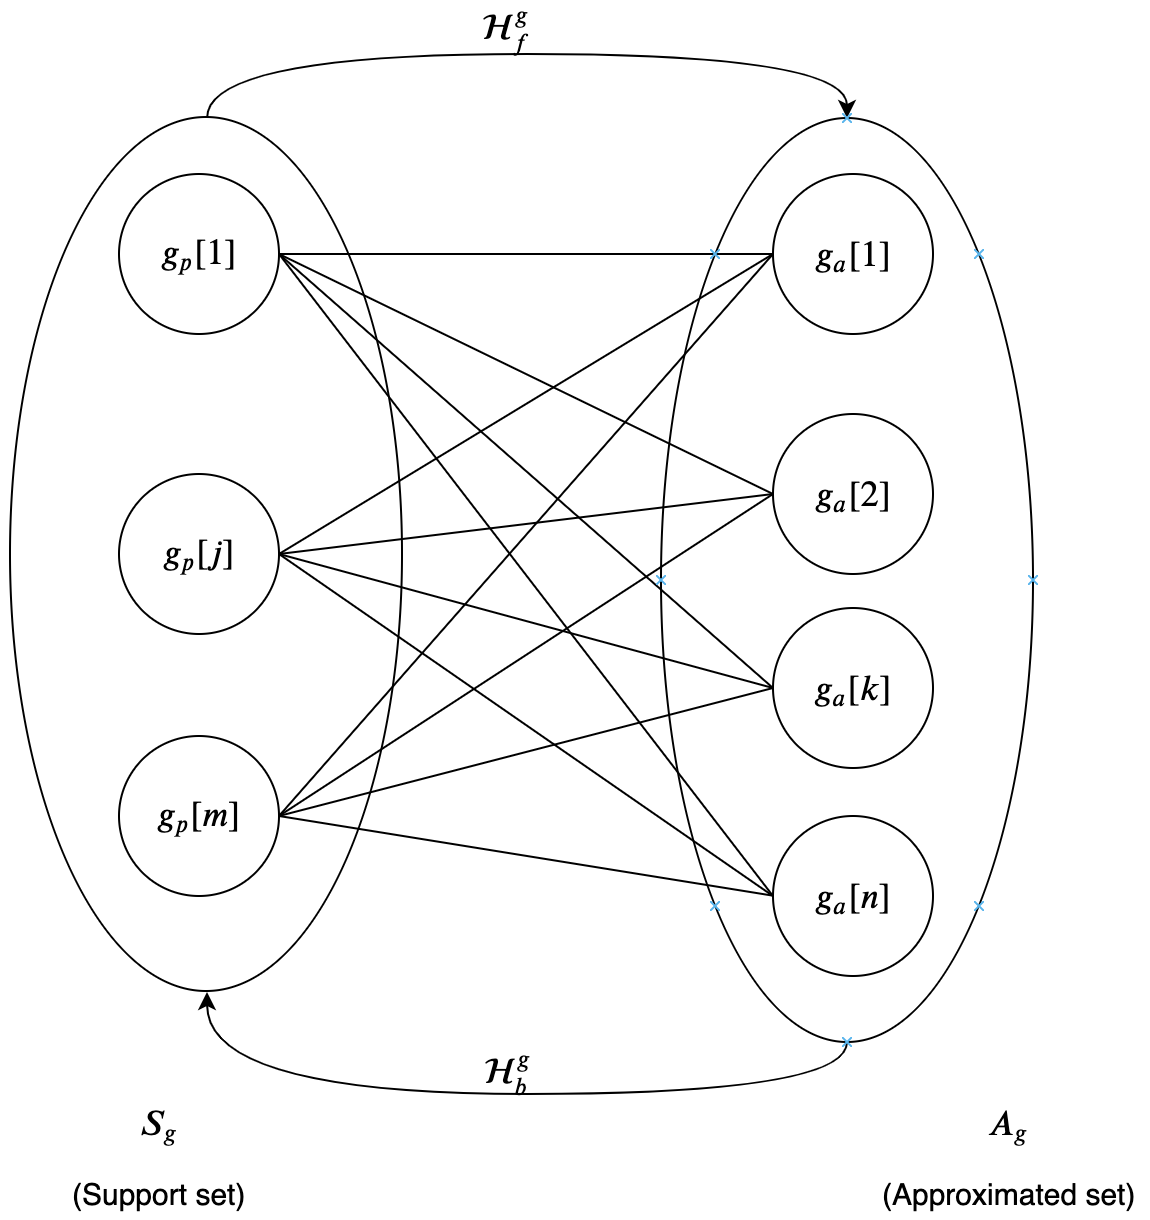
\includegraphics[width=0.47\textwidth]{img/supportApprox.png} %
    \caption{Interaction between Support and Approximated Sets within a group of $m+n$ elements }%
    \label{fig:systemDesign}%
\end{figure}



\subsection{Minimal Support Group}

Next we proceed to find the minimal group that minimizes a set of $l$ objectives $\mathbf{O}=[O_1, O_2, \dots O_l]$ to augment the virtual sensor field physically. 
This solution to such kind of problems is a set of 'non-inferior' solutions where any $O_i$ can not be improved without increasing $O_j , j \neq i$.  
We define two objectives to measure the prediction error due to forward  $\mathcal{H}^g_f$ and backward $\mathcal{H}^g_b$ hypothesis spaces by Equations \ref{eq:fitnessforward} and \ref{eq:fitnessbackward} respectively.
\begin{equation} 
O^v_f (B^c) =\Sigma_{g \in G} \Sigma_{v \in S_g} \Sigma_{u \in A_g} \Big\{ \frac{M^g[\textbf{u,v}]}{|S_g A_g|} \Big\} 
\label{eq:fitnessforward}
\end{equation}
\begin{equation} 
O^v_b (B^c) =\Sigma_{g \in G} \Sigma_{v \in S_g} \Sigma_{u \in A_g} \Big\{ \frac{M^g[\textbf{v,u}]}{|S_g A_g|} \Big\} 
\label{eq:fitnessbackward}
\end{equation}

Next we model the monitory risk associated with a smart building solution as the total number of sensors in $S_g$, cost of the hardware solution and energy consumption of the same.
Let there are two 1D vectors $P^w_g = \{pw_1, pw_2 \dots pw_k\}$ and $P^r_g = \{pr_1, pr_2 \dots pr_k\}$ to store the power consumption and purchase cost respectively. 
Correspondingly Equation \ref{eq:smCost} expresses the cost of implementing smartness in a building as the dot product of encoding and price vector.
Similarly Equations \ref{eq:numSens} and \ref{eq:sbOpCost} infer the number of sensors and power consumption for an arbitrarily encoded sequence respectively. 

\begin{equation}
    O_{cost}  =  \Sigma_{g \in G=Z} <A^c(g), P^r_g> 
    \label{eq:smCost}
\end{equation}
%
\begin{equation}
    O_{\# sens}  = \Sigma_{g \in G=Z} <A^c(g ), \Vec{1}>
    \label{eq:numSens}
\end{equation}
%
\begin{equation}
    O_{energy} =  \Sigma_{g \in G=Z} <A^c(g), P^w_g>
    \label{eq:sbOpCost}
\end{equation}
For a group, we penalize an encoding of all zeroes by Equation \ref{eq:penalty} since it means no sensors are reduced and the learnt hypothesis space is not used.
\begin{equation}
P (A^c(g))=  \begin{cases}
    \infty,& \text{if } A^c(g) = 0_{1 \times |A^c(g)|} \\
    0,    & \text{otherwise}
\end{cases}
\label{eq:penalty}
\end{equation}

Figure \ref{fig:ngisSchematic} depicts the flow chart in which the system optimises the virtual sensor field with a minimal group of sensors. We use NSGA II \cite{deb2002fast} to search the chromosomal vector space of $O(2^{KZ})$ to optimise our objectives. 
\begin{enumerate}
    \item Take as input the learnt hypothesis space and error matrix $\{\mathcal{H}^g, M^g\}  \forall g \in G$.
    \item Initialize a genetic pool ($P_t$) of chromosomes as a random string of 0's and 1's.
    \item For every chromosome, evaluate the objective set $[O^v_f, O^v_b,  O_{cost} ,  O_{\# sens}, O_{energy}]$.
    \item If the maximum number of generations are reached or incremental gain is lower than a threshold the algorithm stops else a child population $Q_t$ is created using steps 5, 6 and 7.
    \item Non dominated sorting is used to incrementally identify Pareto optimal solutions till the entire population is exhausted.
    \item Crowding Distance is used to check the density around individual solutions to prevent the algorithm for terminating in a local optima. In fact, chromosomes that fall within the rectangular field spanned by the nearest adjacent solutions are discarded.
    \item Alteration in the encoding is achieved through genetic operators: Random Crossover and Mutation.  
    \item Now populations $P_t$ and $Q_t$ are combined to generate the parent population at time $t+1$ using steps 5 and 6 in order.
    \item Go back to Step 3 and iterate with generation count decreased by 1.
\end{enumerate}
The algorithm terminates with a set of Pareto optimal solutions or minimal groups. 
We experimentally investigate the quality of these groups that can optimally power up the virtual sensor field.
 \begin{figure}
     \centering
     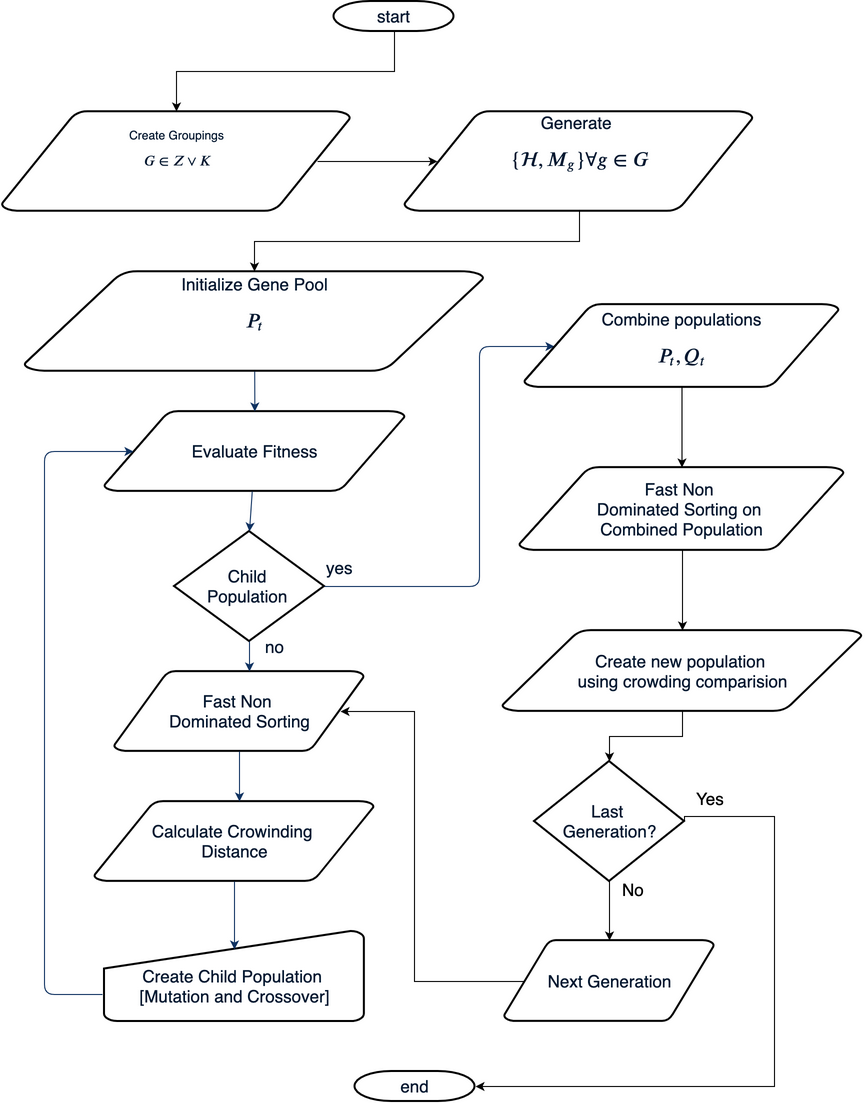
\includegraphics[width=0.5\textwidth]{img/ngisSchematic.png}
     \caption{Sequence of Steps to Optimize the Virtual Sensor Field }
     \label{fig:ngisSchematic}
 \end{figure}
